\cotefile{156-6}
\scanpage{50}
\mspage{49}

\uline{Lemme} Soient $I,I'$ deux ens \deleted{\unsure{part.}}\deleted{\unsure{pré}} ordonnés, Alors l'application
\[
\operatorname{Hom}_{\unsure{\mathrm{croiss}|\mathrm{Croiss}}}(I,I')\longrightarrow
\operatorname{Hom}_{\mathrm{cr}}(\unsure{Pf|P_f}(I'),Pf(I))
\]
entre applications croissantes de $I$ dans $I'$, et appl. cr. de $Pf(I)$ en $Pf(I')$ (parties \deleted{\unsure{ouv.}} fermées de $I,I'$) est \uline{injective}. Son image est formée \deleted{des} de certaines des
\begingroup\csname tagsleft@true\endcsname
\[
Pf(I')\longrightarrow Pf(I)\tag*{$(\unsure{x|\alpha})$}
\]
\endgroup
\unsure{qui}, commutent aux intersections \inserted{et réunions} quelconques \deleted{et aux réunions finies \unsure{(la dernière est kif-kif)}}\unsure{,} et \inserted{\unsure{de} toutes si $I$ est sobre (\uuline{p.ex. $I$ fini})}
% slanted
\margin{Elles commutent alors aux réunions quelconques, et inversement}

\deleted{\unsure{Bien}} Passant aux complémentaires ouverts, \inserted{on voit que} les applications $(x)$ correspondent aux \inserted{\unsure{classes d'is.} des} morphismes \deleted{qui \unsure{sont compatibles aux} \unsure{produits|précédents}} de Topos $\operatorname{Top}(I)\unsure{-|\to}\operatorname{Top}(I')$, \deleted{Mais \unsure{ils ne} \illegible{1}} \inserted{ayant une} propriété suppl. (compatibilité aux intersections \uline{quelconques}) \deleted{$I$ est \unsure{évidemment} \unsure{i.e.} sobre,} Ces \deleted{\unsure{appl}} alors correspondent aux applications continues i.e. croissantes
\[
I\longrightarrow\widehat{I}'
\]
où $\widehat{I}'$ est l'espace sobre associé à $I'$, \unsure{i|;}

\uline{NB} on n'avait pas \unsure{$\prime\prime$|à} supposer $I$ séparé ) \deleted{\unsure{on sait} \unsure{$I$}} \deleted{Comme $\unsure{I'^{\circ}|I'^{0}}\longrightarrow\widetilde{I}'$ ($I'$ séparé) cela donne l'injectivité, et pour la bijectivité \unsure{alors|aussi} quand $I'$ sobre i.e. $I'=\widetilde{I}'$}
% slanted
\margin{transformant les $i\in I$ en des \deleted{\unsure{éléments}} \uline{\unsure{stricts|strict}} de $I'$ \inserted{parties fermées irréductibles donc de la forme $\overline{\{i'\}}=I'_{\leq i'}$ (comme $I'$ séparé, cela signifie $I-I'$ \unsure{quel|que|quelc.}}}

Donc cela nous fournit bien (1.55) \deleted{\unsure{pour}} \deleted{au moins si $I'$ sobre \unsure{p.ex.} $I'$ \unsure{fini}} Mais aura-t-on réciproquement que la top de $\widetilde F$ est image inv. de celle de $\widetilde F'$ ? En fait, c'est \uline{équivalent} à la surjectivité de (1.54).

\uline{Ex} Prenons des ateliers ``triviaux'' (p. 44) définis par $(M,\leq,\ll\overset{\mathrm{dfn}}{=}\leq,F)$. \deleted{\unsure{autrement}}\inserted{\unsure{Simplement|Signalons} ici} \deleted{qui \unsure{fait}) \unsure{$\mathcal F$}} : l'axiome At 8, il signifie que pour tt $X\in M$, $\exists\,x\in M$, $x$ \uline{minimal}, tel que $x\leq X$, \unsure{mais} et que \inserted{dans le cas $X\ne x$ i.e. $X$ non \unsure{mini|minim.}} $X$ soit ``successeur'' de
\scanpage{51}
\mspage{50}
$x$\unsure{''}. i.e. $\nexists\,Y\in M$ \unsure{avec} $x\leq Y<X$. C'est évidemment une condition des plus restrictives sur $M$ ! Passons, et ne nous préoccupons pas de At 8.
% slanted
\margin{``tout élément de $M$ est minimal, ou successeur d'un minimal''. Sous condition des \unsure{chaînes}, cela implique $\dim M\leq1$.}
Considérons \deleted{des} un autre $(M',\leq,\ll\overset{\mathrm{dfn}}{=}\leq,F')$, prenons \deleted{\unsure{tt}} \unsure{pour|pour y} \unsure{faire|fixer} $\unsure{\mathcal F|F|\mathscr F}=\unsure{Pf|P_f}(M)$, $\mathcal F'=Pf(M')$, et intéressons-nous aux
\[
f:F'\longrightarrow F
\]
\deleted{tels} qui soient des morphismes d'ateliers, au sens de la définition p. 47. Par le lemme, ils correspondent aux \deleted{\unsure{hom}} applications croissantes en sens inverse
\diagram{\begin{tikzcd}[ampersand replacement=\&,row sep=small,column sep=2em]
M \arrow[d,"\unsure{\varphi|\psi}"]\\
M' \& {,}
\end{tikzcd}}
sans aucune condition supplémentaire.

Cela montre que la condition que $\varphi$ de (1.55) soit telle que la top. de $\widetilde F$ soit \deleted{\unsure{l'image}} initiale pour $\varphi$, i.e. que (1.54) soit tjrs surjective, est bien substantielle.

\uline{Exemples} 1) Soit $f:L\unsure{-|\to}L'$ application ensembliste, elle induit \deleted{\unsure{Fig}}
\[
\begin{aligned}
f^{\unsure{*|x}}:\operatorname{Fig}(L')&-\operatorname{Fig}(L)\\
\deleted{\unsure{F'|f^{?}}}\deleted{\unsure{A'}}\unsure{\Phi'|\underline{\Phi}'}&\longmapsto\{f^{-1}(A')\mid A'\in\Phi',\, f^{-1}(A')\ne\varnothing\}
\end{aligned}
\]
\scanpage{52}
\mspage{51}
qui est un comorphisme d'ateliers

2) 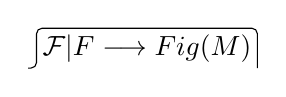
\begin{tikzpicture}[baseline=(v.base)]\node[inner sep=2pt] (v) {$\unsure{\mathcal F|\mathscr F}\longrightarrow\operatorname{Fig}(M)$};\draw[rounded corners=2pt] ([xshift=-3pt]v.south west)--(v.south west)--(v.north west)--(v.north east)--(v.south east);\end{tikzpicture} est un comorphisme d'ateliers injectif, satisfaisant la condition \inserted{de bijectivité} (1.54). En le composant avec des comorphismes \unsure{Fig}
\[
\operatorname{Fig}(M)\unsure{-|\to}\operatorname{Fil}(L)
\]
\unsure{déduit|induit|évident} comme dans $1^\circ$ \unsure{des|de} $L\unsure{\hookrightarrow|\subset}M$, on trouve des comorphismes
\[
\mathcal F-\operatorname{Fig}(L)
\]
\deleted{\unsure{l'un et}}\inserted{comme} l'autre, \inserted{il} satisfont la condition suppl. \inserted{\deleted{\unsure{de}} de bijectivité} (1.54), si cette fois on suppose \uline{At} 8 ; et sans \uline{que} $f$ soit \unsure{néc.} injectif.

\uline{Définition} On dit qu'un comorphisme $f:\mathcal F'\to\mathcal F$ d'ateliers est un co\uline{plongement}, si

\deleted{a) $f$ est injectif}

\deleted{\unsure{b)}}a) l'image $f(\mathcal F')$ est un sous-atelier de $\mathcal F$ \inserted{(p. \unsure{43|47})}
\par b) $f$ induit un iso. $\mathcal F'\unsure{\stackrel{\sim}{-}|\xrightarrow{\sim}}f(\mathcal F')$.
% slanted
\margin{Comparer avec perplexité marginale bas page 47}

\deleted{\unsure{Cel}} Les conditions \unsure{a)} b) équivalent \unsure{(}compte tenu de a) à : \par a') $\forall\,F'\in\mathcal F'$, \inserted{posant $F=f(F')$} l'application
\begingroup\csname tagsleft@true\endcsname
\[
\operatorname{Sousfig}(F')\longrightarrow\operatorname{Sousfig}(F)\qquad G'\unsure{\mapsto|-} f(G')\tag*{$(*)$}
\]
\endgroup
est bijective, \inserted{ou seulement} \deleted{\unsure{i.e.}}\deleted{\unsure{(comme}} elle est déjà injective par l'inj. de $f$, qui résulte de b) la surjectivité :
\[
\forall\,G\leq F,\ \exists\,G'\leq F'\quad\text{telle que}\quad G^{\unsure{*}}=f(G').
\]

b') $\forall\, F',\deleted{\unsure{F}}G'\deleted{\unsure{F|G}},\in \unsure{F'|\mathcal F'}$, on a
\[
f(G')\ll f(F')\Longrightarrow G'\ll F'
\]
% slanted
\margin{\uline{NB} Si $f$ est injective, alors $\mathrm{a}')\Rightarrow\mathrm{a})$, cf plus bas.}
\scanpage{53}
\mspage{52}

\inserted{C'est évidemment nécessaire. Pour la suffisance,} Il suffit de voir que \deleted{\unsure{cela implique}} les conditions a') b'), \deleted{\unsure{a)}} impliquent, \inserted{$f$ injectif (ce qui résulte de b') et que} pour $F',G'\in\unsure{\mathcal F'|\mathscr F'}$
\[
f(G')\leq f(F')\Longrightarrow G'\leq F'
\]

\uline{Dém} \deleted{\unsure{Par}} b'), \deleted{$\unsure{\exists\,G'}$} si $f(G')\leq f(F')$, $\exists\,\overline{G'}\leq F'$ tel que $f(\overline{G'})\deleted{\unsure{\leq}}=f(G')$. Mais alors par a on a $G'=\overline{G'}$, d'où $G'\leq F'$, \unsure{q.e.d.|p.c.d.}

\uline{Définition} On dit que l'atelier $\mathcal F$ \inserted{(satisfaisant At 1--At 8)} est \deleted{\unsure{faiblement}} \inserted{\uline{quasi}} \uline{ensembliste} (on renforcera ce ``ensembliste'' plus tard) si le comorphisme canonique
\[
\mathcal F\unsure{-|\to}\operatorname{Fig}(L)
\]
est un \uline{plongement}, ou, ce qui revient au $\unsure{=|<}$ (compte tenu de (1.53) p. 46) si on a
% slanted
\margin{Pour correctif voir \unsure{CF|GF} 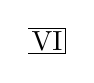
\begin{tikzpicture}[baseline=(n.base)]\node[inner sep=1pt] (n) {$\mathrm{VI}$};\draw (n.north west)--(n.north east)--(n.south east)--(n.south west);\end{tikzpicture} p. 12}
\[
\begin{aligned}
\text{\uuline{At ens 1}}\qquad &\forall\, F,G\in\mathcal F,\\
&\unsure{\operatorname{mulomb}|\operatorname{mulom}}(F)\ll\operatorname{mulomb}(G)\Longrightarrow F\ll G.
\end{aligned}
\]

\uline{Remarque} 1) On voit qu'il suffit de poser At ens 1 pour $F,G$ des multistrates $X,Y\in M$. Ce serait plus joli de poser At ens en ces termes.

2) On n'exige pas que le sous-atelier $\mathcal F\hookrightarrow\operatorname{Fig}(L)$ soit \unsure{gracieux|spacieux}. \uline{Par \unsure{exemples|exemple}} \deleted{\unsure{Considérons}} \deleted{de \unsure{l'exemple} \unsure{$B$}} \deleted{\unsure{C)}} Soit $E$ un espace topologique ou modéré, et $M$ l'ens de ses \uline{m}ultistrates \uline{simplexes} (topologiques, ou modérés), mais
\scanpage{54}
\mspage{53}
\unsure{Contrairement|(contrairement} à l'exemple B) p. 34) sans structure affine. On définit la compatibilité des simplexes comme dans loc. cit. \deleted{Mais \unsure{ce n'est pas} c'est}
D'où \unsure{ens} de multistrates, \unsure{on prendra|où pour des} $\unsure{\mathcal F|\mathscr F}$ \unsure{ensemble|en met} des \deleted{multistrates}\inserted{simplexes} fermé\deleted{\unsure{e|es}}s pour $\leq$, et formés de simplexes deux à deux compatibles. L'axiome A 8 \unsure{trivialmt|trivialement} valable (NB \deleted{\unsure{$L$}}$E$ s'identifie à $L$). Mais la notion de compatibilité des simplexes est plus fine que la compatibilité des figures ensemblistes associées -- puisqu'ici on exige \inserted{de plus} que la figure intersection soit élémentaire, i.e. soit une multistrate commune. On y reviendra par la suite\ldots

Ainsi, dans le cas d'un atelier ensembliste, $\mathcal F$, $\mathcal F$ se réconstitue à partir de \deleted{\unsure{un}} l'ens des figures \unsure{dans|des} $\unsure{\mathcal L|L}$ qu'il décrit, comme sous-atelier de $\operatorname{Fig}(L)$. La question est donc \uline{quels} sous-ateliers d'un ens $L$ on obtient ainsi.
\scanpage{55}
\mspage{54}

\uline{Scholie} Se donner un atelier (quasi) ensembliste, ``revient au $=$'' que de se donner un couple $(L,\unsure{\mathcal F|\mathscr F})$, où $L$ est un ens, $\mathcal F$ un sous-atelier de $\operatorname{Fig}(L)$, satisfaisant \unsure{la|les} condition\deleted{\unsure{s}} suivante\deleted{\unsure{s}} :

\deleted{\uline{At ens$^{*}$ 1} \deleted{\unsure{(sé)|(sép.)|(*)}} Les strates des $\unsure{\Phi|\underline{\Phi}}\in\mathcal F$ séparent les points de $L$, i.e. si $x,y\in L$, $x\ne y$, alors $\exists\,\deleted{\unsure{\Phi}}\unsure{P|F}\in\Phi$, $A\in \unsure{P|F}$, tel qu'on ait $x\in A$, $y\notin A$ ou $y\in A$, $x\notin A$.}

\[
\text{\uline{At ens}}^{*}\,\deleted{\unsure{2}}1\quad \deleted{\unsure{\varnothing .}}\quad
\forall\,x\in L,\quad\{\{x\}\}\in\mathcal F
\]

\deleted{\unsure{Le}} Le tout est de vérifier que, dans ce cas, $L$ se réconstitue à partir de $(\mathcal F,\leq,\ll)$ comme l'ens des lieux de $\mathcal F$, donc que
\[
x\longmapsto\{\{x\}\}=\Phi_x
\]
est une bijection de $L$ \deleted{\unsure{(ou de $M$}}\inserted{avec} l'ens des éléments de $\mathcal F\setminus\{\varnothing\}$ minimaux pour $\ll$. \inserted{Il est clair que $\Phi_x$ est minimal dans $\operatorname{Fig}(L)\setminus\unsure{\{\varnothing\}|(\varnothing)}$, a fortiori dans $\mathcal F\setminus\{\varnothing\}$}.

Or soit $F\in\deleted{\unsure{\Phi}}\mathcal F\setminus\{\varnothing\}$, \inserted{minimal} \deleted{Soit $A\in F$, on a $A^{\circ}\ne\varnothing$, soit $x\in A^{\circ}$ alors $\Phi$} \deleted{Soit} On a $|F|\ne\varnothing$ (puisque $F\ne\varnothing$) soit $x\in |F|$, alors $\Phi_x\ll F$, donc $\Phi_x=F$, cqfd.
\scanpage{56}
\mspage{55}

Je rappelle pour mémoire les conditions \inserted{Sous at 1,2} \inserted{de page 42} pour qu'une partie ${\unsure{\mathcal F|\mathscr F}}^{\unsure{f|*|\prime}}$ de $\operatorname{Fig}(L)$ (en l'occurrence) :

\uline{At ens$^{*}$} 2 \quad $\mathcal F$ est fermé dans $\operatorname{Fig}(L)$ pour $\leq$, i.e. si $F\in\mathcal F$, alors \unsure{toute|tt} sous figure de $F$ est dans $F$.

\uline{At ens$^{*}$} 3 \quad Si $F,G\in\mathcal F$, et si pour \deleted{pour \unsure{tte} $F$ et $G$ sont compat} toute multistrate $F_A$ de $F$, $G_B$ de $G$, $\{F_A\unsure{,|\vee}G_B\}$ est majoré dans $\mathcal F$, \inserted{i.e. $F_A\mathrel{\vcenter{\hbox{
\begin{tikzpicture}[x=1ex,y=1ex,baseline]\draw (0,0)--(1.05,.50)--(0,1);\draw (1.05,0)--(0,.50)--(1.05,1);\end{tikzpicture}}}}G_A$ et $F_A\unsure{\dot\vee|\vee}G_A\in\mathcal F$} \deleted{alors} \inserted{(a fortiori les figures \deleted{\unsure{ou}} $F,G$ sont \inserted{alors} \unsure{ensemblistmt} compatibles)} \deleted{$F,G$} $F\vee G\in\mathcal F$.

Ceci peut s'expliciter \unsure{aussi|ainsi} \inserted{(partiellement)} en termes d'un ensemble $M$ de figures \inserted{(ensemblistes)} élémentaires dans $L$, \deleted{\unsure{en convenant pour} $\mathcal F$} \inserted{avec une} relation $\underset{M}{\mathrel{\vcenter{\hbox{
\begin{tikzpicture}[x=1ex,y=1ex,baseline]\draw (0,0)--(1.05,.50)--(0,1);\draw (1.05,0)--(0,.50)--(1.05,1);\end{tikzpicture}}}}}$ (``compatibilité géométrique'') \inserted{réfl. et sym} dans $M$, satisfaisant les conditions

\[
\big|\,\text{\uline{At ens}}\ \unsure{\sharp|\mathrm{gf}|{}^{**}}\ 1\qquad\forall\,x\in L,\quad\{\{x\}\}\in M
\]

\noindent\raisebox{0pt}[0pt][0pt]{\rule[-1.5\baselineskip]{.35pt}{2.4\baselineskip}}\quad
\uline{At ens} $\sharp$ 2 \quad \deleted{\unsure{$A$}} $\forall\,X\in M$, toute sous-multistrate est dans $M$

\noindent\raisebox{0pt}[0pt][0pt]{\rule[-2.1\baselineskip]{.35pt}{3\baselineskip}}\quad
\uline{At ens} $\deleted{{}^{**}}\sharp$ 3 \quad Si $X,Y\in M$ et $X\underset{M}{\mathrel{\vcenter{\hbox{
\begin{tikzpicture}[x=1ex,y=1ex,baseline]\draw (0,0)--(1.05,.50)--(0,1);\draw (1.05,0)--(0,.50)--(1.05,1);\end{tikzpicture}}}}}Y$, et $X',\deleted{\unsure{Y'}}\leq X$, $Y'\leq Y$, alors $X'\underset{M}{\mathrel{\vcenter{\hbox{
\begin{tikzpicture}[x=1ex,y=1ex,baseline]\draw (0,0)--(1.05,.50)--(0,1);\draw (1.05,0)--(0,.50)--(1.05,1);\end{tikzpicture}}}}}Y'$ ; de plus $X\underset{M}{\mathrel{\vcenter{\hbox{
\begin{tikzpicture}[x=1ex,y=1ex,baseline]\draw (0,0)--(1.05,.50)--(0,1);\draw (1.05,0)--(0,.50)--(1.05,1);\end{tikzpicture}}}}}Y\Longrightarrow X\underset{\mathrm{ens}}{\mathrel{\vcenter{\hbox{
\begin{tikzpicture}[x=1ex,y=1ex,baseline]\draw (0,0)--(1.05,.50)--(0,1);\draw (1.05,0)--(0,.50)--(1.05,1);\end{tikzpicture}}}}}Y$
\scanpage{57}
\mspage{56}

On trouve

\uline{Scholie} des ateliers \inserted{(quasi)} ensemblistes à figures de type fini : se donner un tel atelier, revient au $=$ que de se donner un \deleted{\unsure{ens}} couple $(L,M)$, $L$ ensemble, $M$ ens. de figures élémentaires dans $L$, telles que toute sous figure $F$ d'un $X\in M$ soit de type fini (OK si les $X\in M$ sont des figures finies) et satisfaisant de plus At ens $\unsure{\sharp|\mathrm{gf}|{}^{**}}$ 1 -- At ens $\sharp$ 3.

On \unsure{réconstitut|réconstitue} $\unsure{\mathcal F|\mathscr F}$ comme sous-atelier de $\operatorname{Fig}(L)$, formé des figures \inserted{ens.} \uline{de type fini} telles que \unsure{les|ses} \unsure{multistrates} soient dans $M$.

Dans le cas d'un atelier ens. pas \unsure{néc.} \inserted{à fig.} de type fini, on \deleted{\unsure{préciserait|paraîtrait|présumerait} néanmoins que}
\deleted{pour une figure ensembliste $F$ dans $L$, dont les \deleted{strates} multistrates sont dans $M$, l'appartenance à $\mathcal F$ ne dépend que de son \uline{ombre}.}
